\chapter{Results \& Conclusions}

Now that that all the technical things are done we can run our algorithm to see its accuracy.\newline\newline
For empirical purposes, the algorithm have been run with different train-set and with different settings (e.g. complexity parameter), in order to see the differences between an analysis with and without principal components.\newline
Before showing the results here there are some technical data:\newline

The complexity parameter for the tree construction was set to 0.01, 0.0025 and 0.001 and train-sets were:\newline

\begin{itemize}
	\item[1)] Standardized set, using all the features
	\item[2)] Standardized set, using only the features \emph{selected} by PCA (that is, indeed, a non-standard use of this technique)
	\item[3)] The new set of features \emph{produced} by PCA
\end{itemize}

Regarding test and train set:

\begin{itemize}
	\item The train-set is the 10\% of the Kddcup dataset (which is much much lower than the "standard" dimension, which usually is around 70/80\%)
	\item The test-set is the \emph{whole} Kddcup dataset, consisting of 42 features with almost 5 millions values
	\item When the PCA train-set was used, the test-set was transformed accordingly to the transformations done on the test-set (remember we had to "fit" the scaler with pandas?)
\end{itemize}

Results and some of the plots are shown in the next figures:


\begin{center}
	{\setlength{\extrarowheight}{20pt}
	\begin{tabular}{| c | c | c | c |}
	\hline
		Complexity parameter & 0.01 & 0.0025 & 0.001 \\ \hline
		StandardizedKddcup & 0.9870385 & 0.9832191 & 0.9843356 \\ \hline
		KddcupPrincipalFeatures & 0.9849946 & 0.9948412 & 0.9963878 \\ \hline
		PCA eigenvectors & 0.9901552 & 0.9951242 & 0.9956888 \\ 
		\hline
	\end{tabular}}
\end{center}

\vspace{0.3cm}

If we observe data we can see how Principal Component Analysis raises the accuracy of our prediction. Moreover, the trees built using the selected components are much more balanced when we increase the complexity parameter (i.e. we build bigger trees), while using all the features we get an unbalanced tree.\newline\newline
Another thing to point out is that, with a c.p. of 0.001 we get more accuracy if we don't use the new features produced by PCA (but this could be a matter of the dimension of the train-set)\newline\newline
To conclude, it has been observed that PCA is indeed a useful technique to improve the overall accuracy of predictions in Decision Trees (and it also fasten execution time since we have less features!). For future works, considerations may be done regarding Random Forest (i.e. Distributed IDS) and how to combine it with PCA.\newline\newline
\clearpage
In the following pages there are some plots of the various Decision Tree in order to appreciate the differences between the ones that used PCA and the ones that didn't.
\vspace{2cm}

\begin{itemize}


	\item[Figure 1 - ]This is the tree built with the whole features-set, with a c.p. = 0.0025. As can be seen it is very unbalanced. The more complex is the model, the more unbalanced is the tree


	\item[Figure 2 - ]This is the tree built using the new features produced by PCA. Compared to the previous one, it is much more balanced (and accurate!)


	\item[Figure 3 - ]Just for some fun, this is the (very big) tree, built using PCA's features with a c.p. = 0.001


	\item[Figure 4 - ]And here it is the DT built with the whole feature-set and a c.p. = 0.001. As can be seen, things exhacerbate when we try to build complex models, while using PCA we get better data structures	
\end{itemize}

\clearpage
\afterpage{
\begin{minipage}{\linewidth}
Figure 1
	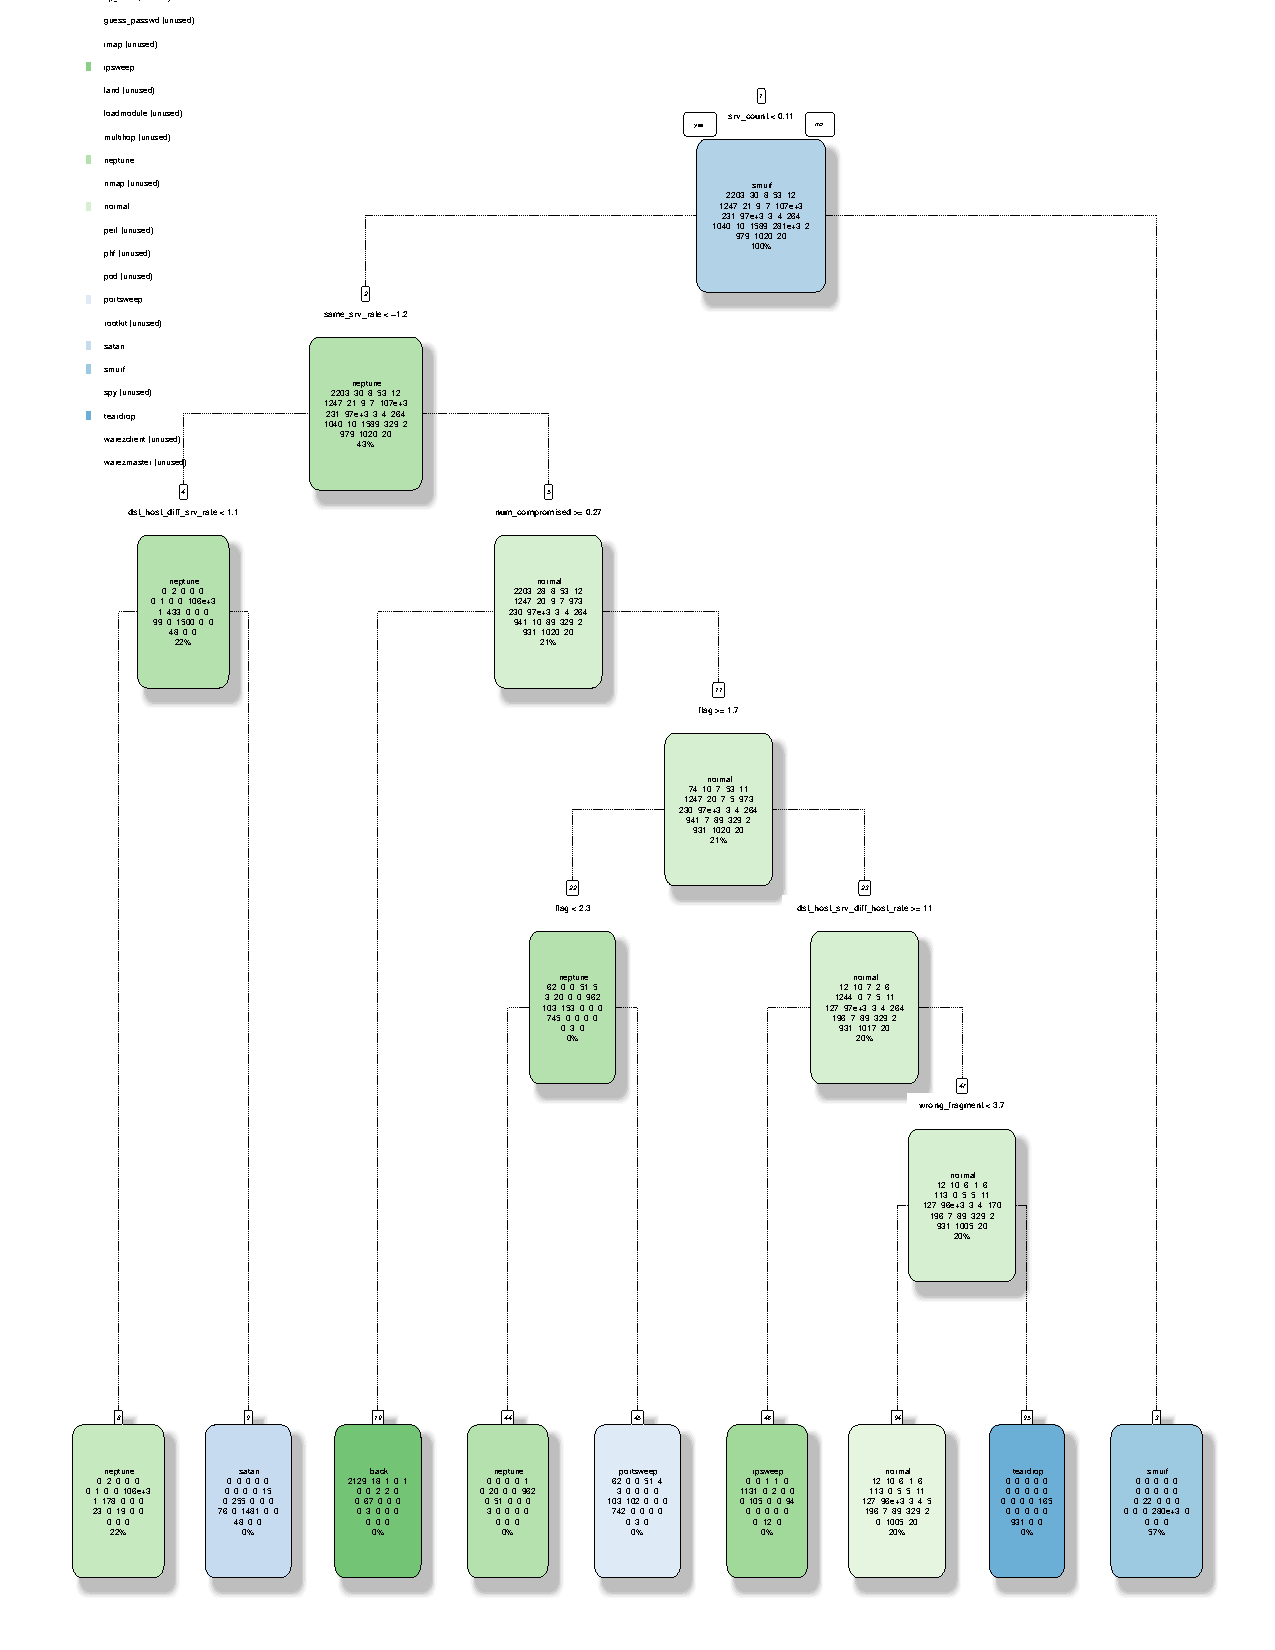
\includepdf{img/noncomponents0025.pdf}
\end{minipage}
}
\clearpage
\afterpage{
\begin{minipage}{\linewidth}
Figure 2
	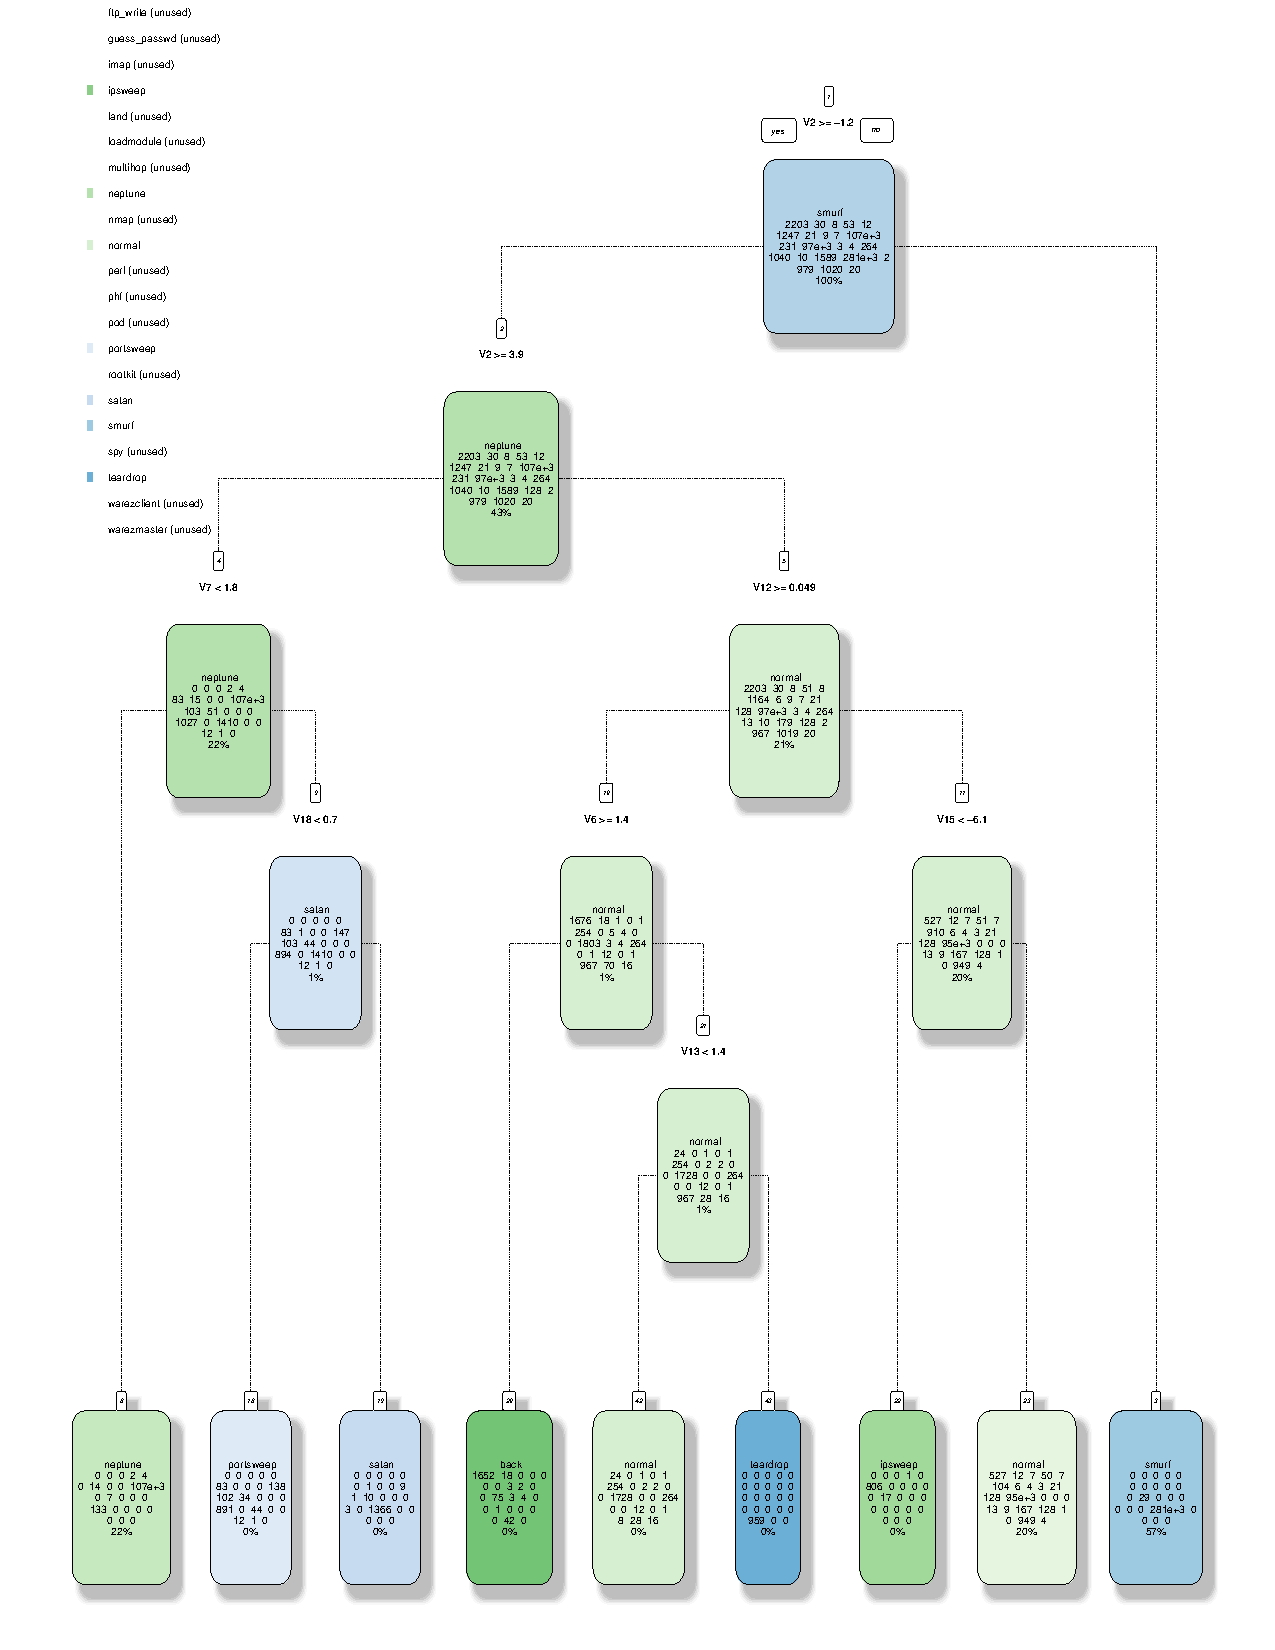
\includepdf{img/components0025.pdf}
\end{minipage}
}
\clearpage
\afterpage{
\begin{minipage}{\linewidth}
Figure 3
	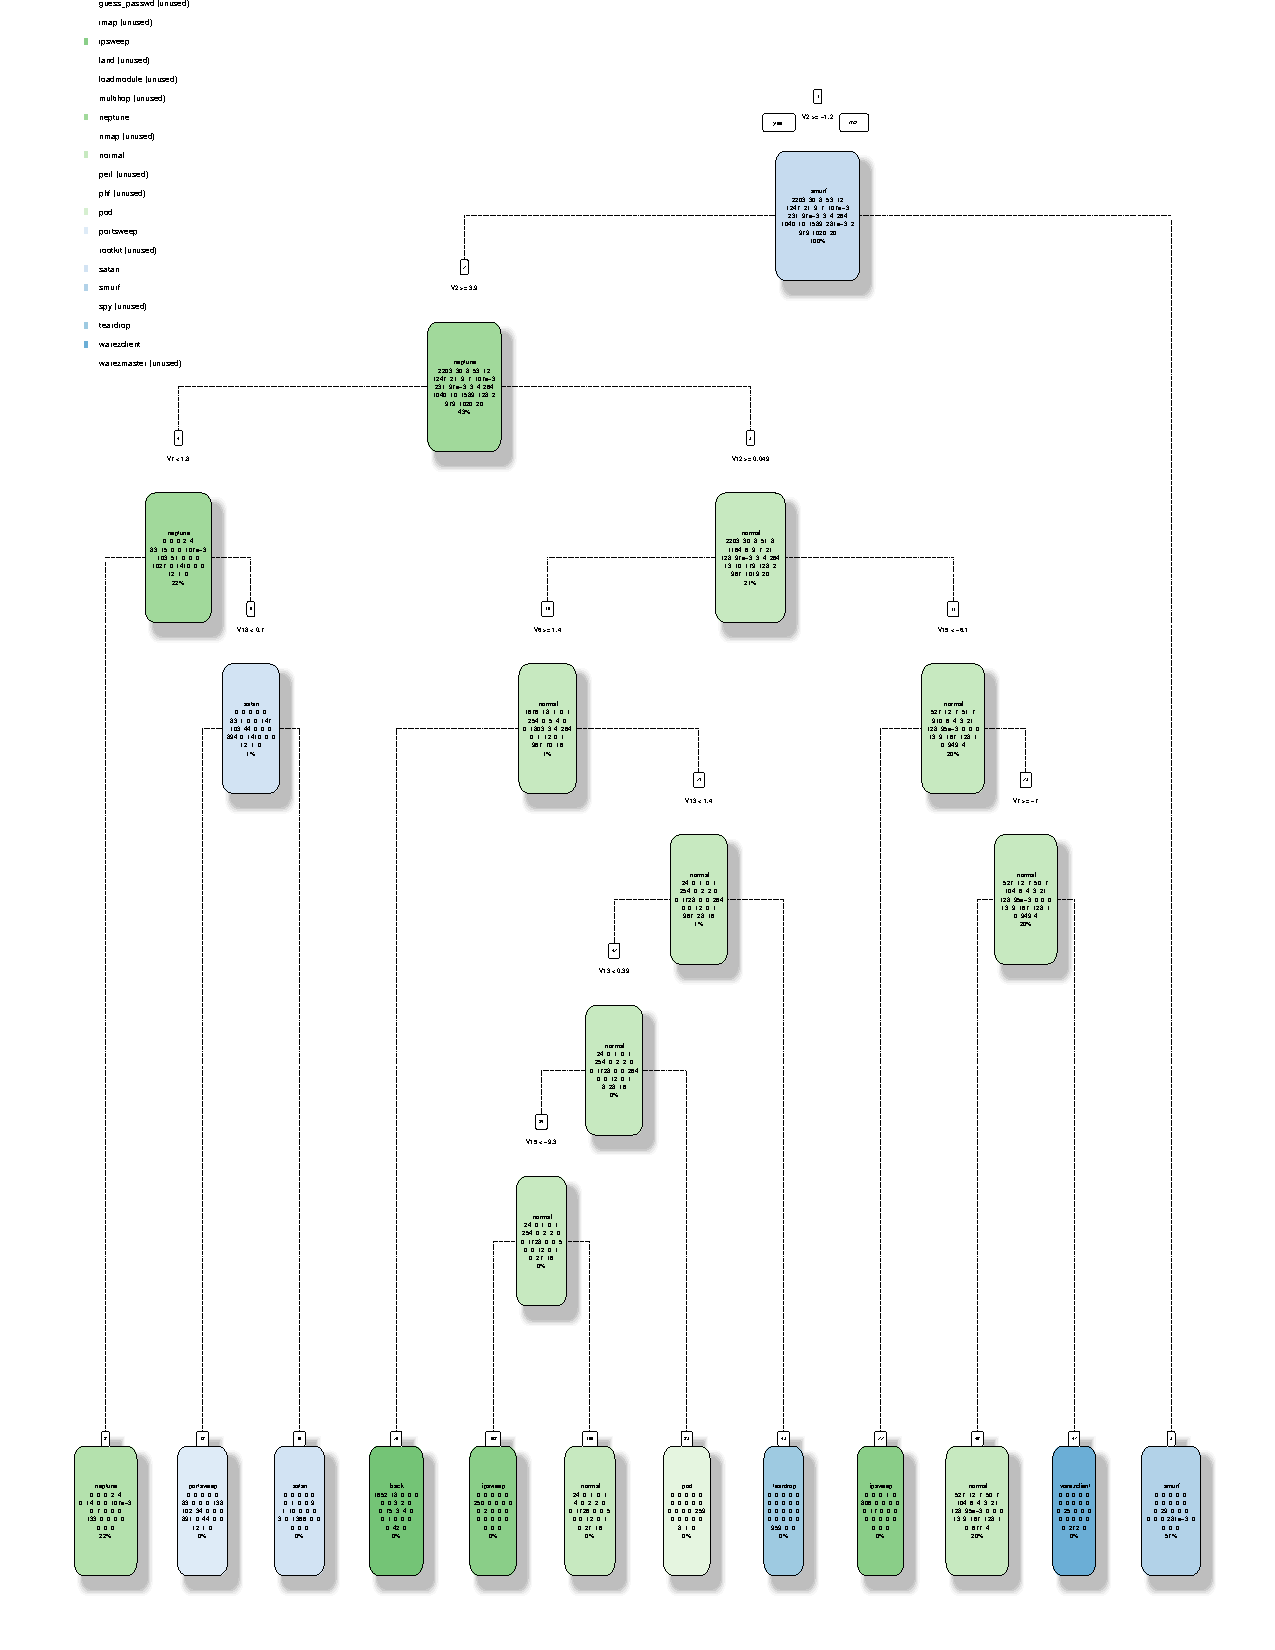
\includepdf{img/components001.pdf}
\end{minipage}
}
\clearpage
\afterpage{
\begin{minipage}{\linewidth}
Figure 4
	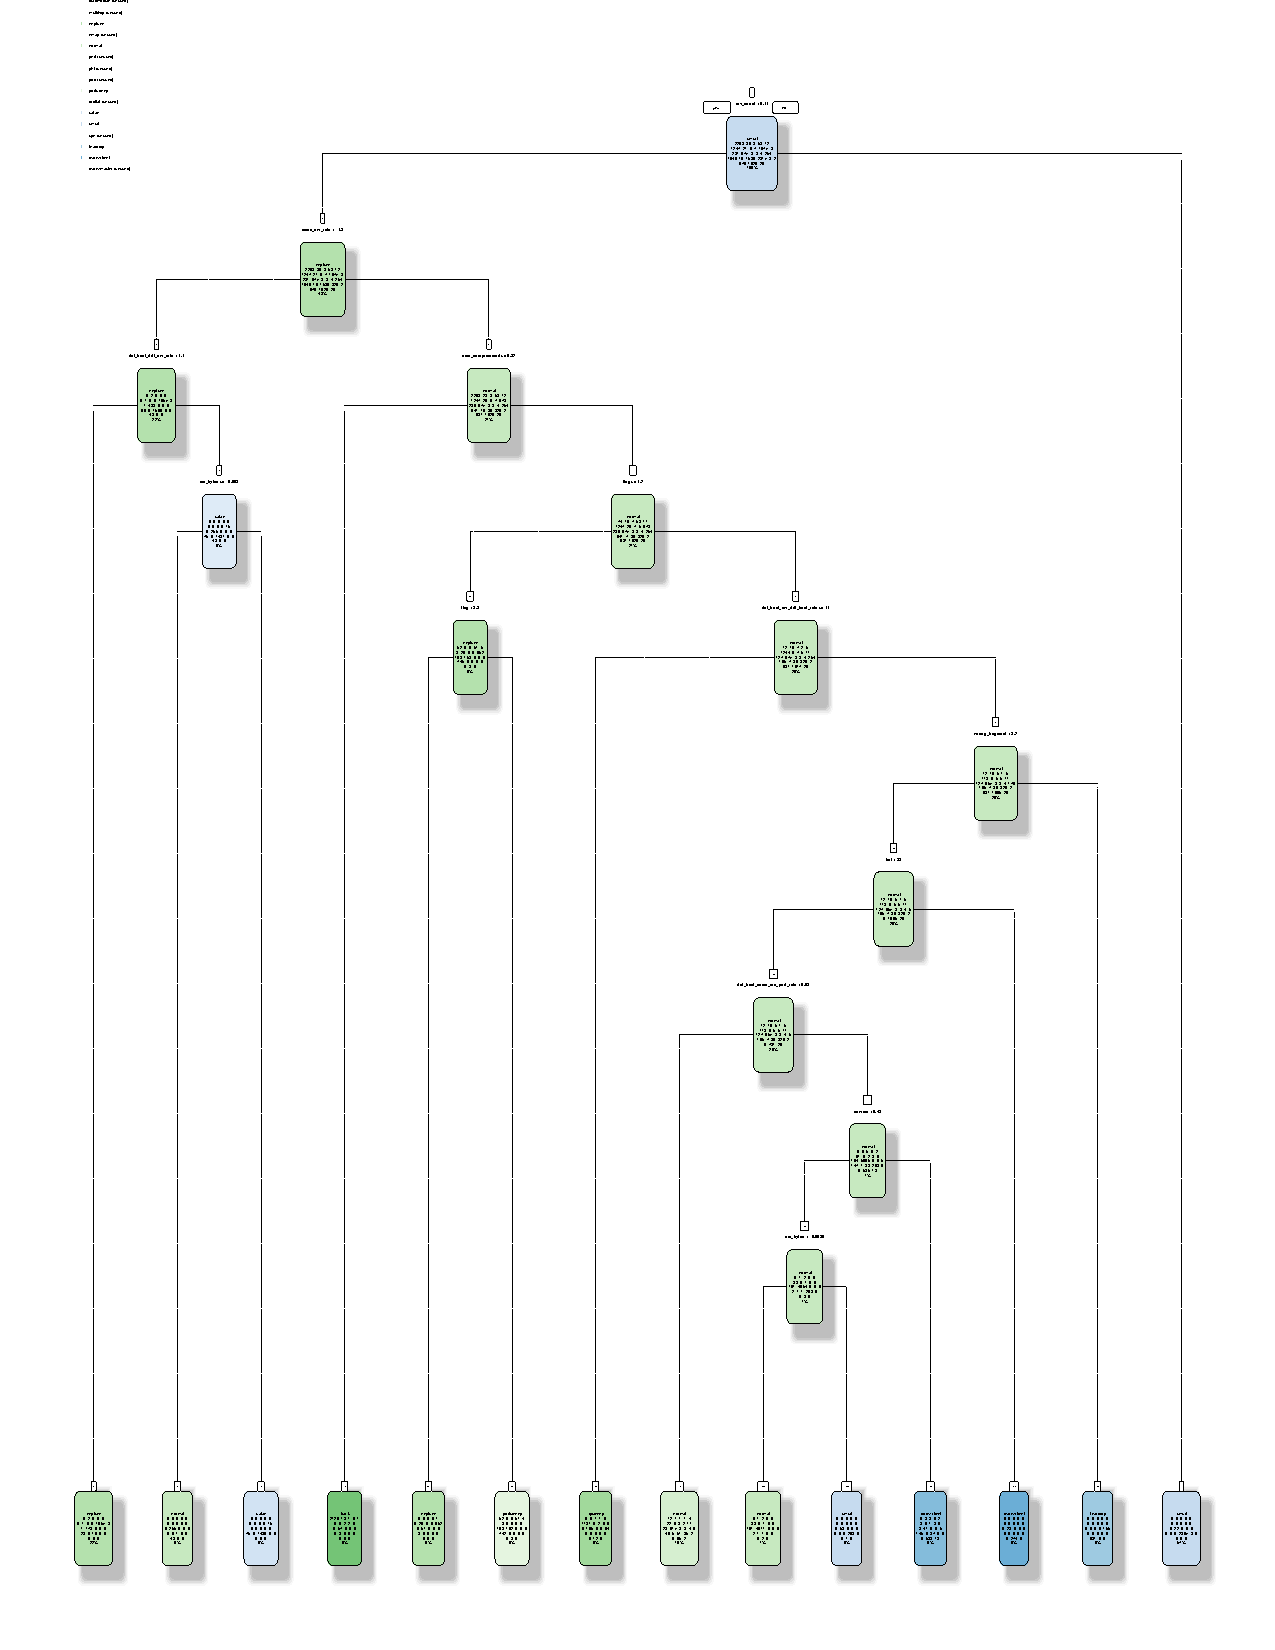
\includepdf{img/noncomponents001.pdf}
\end{minipage}
}